\documentclass{article}
\usepackage{tikz}
\usetikzlibrary{shapes,arrows,positioning,fit,backgrounds,calc,decorations.pathreplacing}
\usepackage{xcolor}

% Define colors
\definecolor{derColor}{RGB}{70,130,180}    % Steel Blue
\definecolor{pmColor}{RGB}{60,179,113}     % Medium Sea Green
\definecolor{protoColor}{RGB}{255,140,0}   % Dark Orange
\definecolor{coordColor}{RGB}{147,112,219} % Medium Purple
\definecolor{reqColor}{RGB}{220,20,60}     % Crimson
\definecolor{evalColor}{RGB}{46,139,87}    % Sea Green

\begin{document}

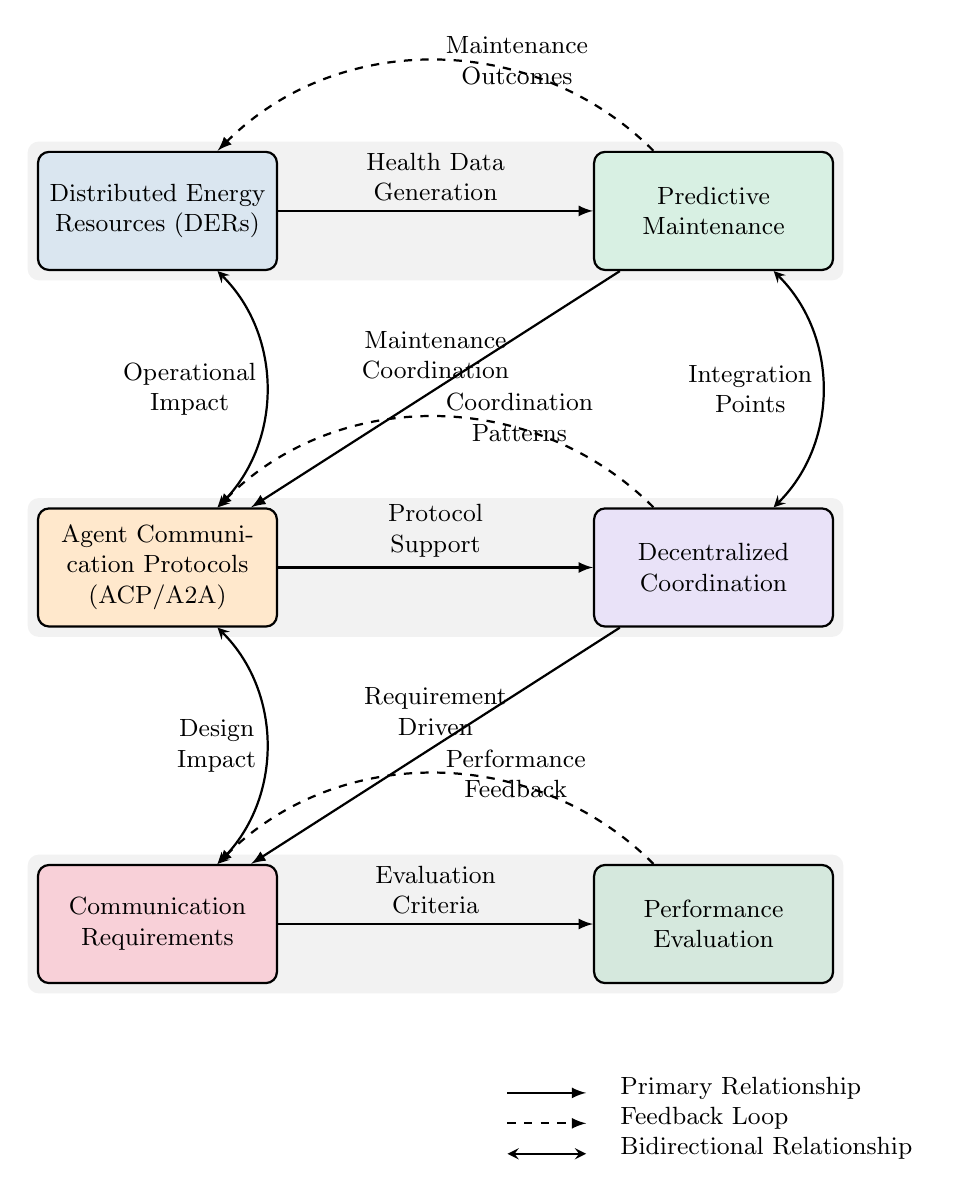
\begin{tikzpicture}[
    node distance=2cm,
    concept/.style={
        rectangle,
        rounded corners,
        minimum width=3cm,
        minimum height=1.5cm,
        text width=2.8cm,
        align=center,
        draw=black,
        thick,
        font=\small
    },
    relationship/.style={
        -latex,
        thick,
        >=stealth
    },
    feedback/.style={
        -latex,
        thick,
        >=stealth,
        dashed
    },
    label/.style={
        font=\small,
        align=center
    }
]

% Main concepts
\node[concept, fill=derColor!20] (der) {Distributed Energy Resources (DERs)};
\node[concept, fill=pmColor!20, right=4cm of der] (pm) {Predictive Maintenance};
\node[concept, fill=protoColor!20, below=3cm of der] (proto) {Agent Communication Protocols (ACP/A2A)};
\node[concept, fill=coordColor!20, right=4cm of proto] (coord) {Decentralized Coordination};
\node[concept, fill=reqColor!20, below=3cm of proto] (req) {Communication Requirements};
\node[concept, fill=evalColor!20, right=4cm of req] (eval) {Performance Evaluation};

% Primary relationships
\draw[relationship] (der) -- node[above, label] {Health Data\\Generation} (pm);
\draw[relationship] (pm) -- node[above, label] {Maintenance\\Coordination} (proto);
\draw[relationship] (proto) -- node[above, label] {Protocol\\Support} (coord);
\draw[relationship] (coord) -- node[above, label] {Requirement\\Driven} (req);
\draw[relationship] (req) -- node[above, label] {Evaluation\\Criteria} (eval);

% Feedback loops
\draw[feedback] (eval) to[bend right=45] node[right, label] {Performance\\Feedback} (req);
\draw[feedback] (coord) to[bend right=45] node[right, label] {Coordination\\Patterns} (proto);
\draw[feedback] (pm) to[bend right=45] node[right, label] {Maintenance\\Outcomes} (der);

% Bidirectional relationships
\draw[relationship, <->] (der) to[bend left=45] node[left, label] {Operational\\Impact} (proto);
\draw[relationship, <->] (pm) to[bend left=45] node[left, label] {Integration\\Points} (coord);
\draw[relationship, <->] (proto) to[bend left=45] node[left, label] {Design\\Impact} (req);

% Background grouping
\begin{scope}[on background layer]
    \node[fit=(der) (pm), fill=gray!10, rounded corners] {};
    \node[fit=(proto) (coord), fill=gray!10, rounded corners] {};
    \node[fit=(req) (eval), fill=gray!10, rounded corners] {};
\end{scope}

% Legend
\node[below=1cm of eval, align=left, font=\small] {
    \begin{tabular}{ll}
        \tikz\draw[relationship] (0,0) -- (1,0); & Primary Relationship \\
        \tikz\draw[feedback] (0,0) -- (1,0); & Feedback Loop \\
        \tikz\draw[relationship, <->] (0,0) -- (1,0); & Bidirectional Relationship
    \end{tabular}
};

\end{tikzpicture}

\end{document} 